\PassOptionsToPackage{unicode=true}{hyperref} % options for packages loaded elsewhere
\PassOptionsToPackage{hyphens}{url}
%
\documentclass[]{article}
\usepackage[a4paper, total={6in, 8in}]{geometry}
\usepackage[UTF8]{ctex}
\usepackage{lmodern}
\usepackage{amssymb,amsmath}
\usepackage{ifxetex,ifluatex}
\usepackage{fixltx2e} % provides \textsubscript
\ifnum 0\ifxetex 1\fi\ifluatex 1\fi=0 % if pdftex
  \usepackage[T1]{fontenc}
  \usepackage[utf8]{inputenc}
  \usepackage{textcomp} % provides euro and other symbols
\else % if luatex or xelatex
  \usepackage{unicode-math}
  \defaultfontfeatures{Ligatures=TeX,Scale=MatchLowercase}
\fi
% use upquote if available, for straight quotes in verbatim environments
\IfFileExists{upquote.sty}{\usepackage{upquote}}{}
% use microtype if available
\IfFileExists{microtype.sty}{%
\usepackage[]{microtype}
\UseMicrotypeSet[protrusion]{basicmath} % disable protrusion for tt fonts
}{}
\IfFileExists{parskip.sty}{%
\usepackage{parskip}
}{% else
\setlength{\parindent}{0pt}
\setlength{\parskip}{6pt plus 2pt minus 1pt}
}
\usepackage{hyperref}
\hypersetup{
            pdfborder={0 0 0},
            breaklinks=true}
\urlstyle{same}  % don't use monospace font for urls
\usepackage{color}
\usepackage{fancyvrb}
\newcommand{\VerbBar}{|}
\newcommand{\VERB}{\Verb[commandchars=\\\{\}]}
\DefineVerbatimEnvironment{Highlighting}{Verbatim}{commandchars=\\\{\}}
% Add ',fontsize=\small' for more characters per line
\newenvironment{Shaded}{}{}
\newcommand{\AlertTok}[1]{\textcolor[rgb]{1.00,0.00,0.00}{\textbf{#1}}}
\newcommand{\AnnotationTok}[1]{\textcolor[rgb]{0.38,0.63,0.69}{\textbf{\textit{#1}}}}
\newcommand{\AttributeTok}[1]{\textcolor[rgb]{0.49,0.56,0.16}{#1}}
\newcommand{\BaseNTok}[1]{\textcolor[rgb]{0.25,0.63,0.44}{#1}}
\newcommand{\BuiltInTok}[1]{#1}
\newcommand{\CharTok}[1]{\textcolor[rgb]{0.25,0.44,0.63}{#1}}
\newcommand{\CommentTok}[1]{\textcolor[rgb]{0.38,0.63,0.69}{\textit{#1}}}
\newcommand{\CommentVarTok}[1]{\textcolor[rgb]{0.38,0.63,0.69}{\textbf{\textit{#1}}}}
\newcommand{\ConstantTok}[1]{\textcolor[rgb]{0.53,0.00,0.00}{#1}}
\newcommand{\ControlFlowTok}[1]{\textcolor[rgb]{0.00,0.44,0.13}{\textbf{#1}}}
\newcommand{\DataTypeTok}[1]{\textcolor[rgb]{0.56,0.13,0.00}{#1}}
\newcommand{\DecValTok}[1]{\textcolor[rgb]{0.25,0.63,0.44}{#1}}
\newcommand{\DocumentationTok}[1]{\textcolor[rgb]{0.73,0.13,0.13}{\textit{#1}}}
\newcommand{\ErrorTok}[1]{\textcolor[rgb]{1.00,0.00,0.00}{\textbf{#1}}}
\newcommand{\ExtensionTok}[1]{#1}
\newcommand{\FloatTok}[1]{\textcolor[rgb]{0.25,0.63,0.44}{#1}}
\newcommand{\FunctionTok}[1]{\textcolor[rgb]{0.02,0.16,0.49}{#1}}
\newcommand{\ImportTok}[1]{#1}
\newcommand{\InformationTok}[1]{\textcolor[rgb]{0.38,0.63,0.69}{\textbf{\textit{#1}}}}
\newcommand{\KeywordTok}[1]{\textcolor[rgb]{0.00,0.44,0.13}{\textbf{#1}}}
\newcommand{\NormalTok}[1]{#1}
\newcommand{\OperatorTok}[1]{\textcolor[rgb]{0.40,0.40,0.40}{#1}}
\newcommand{\OtherTok}[1]{\textcolor[rgb]{0.00,0.44,0.13}{#1}}
\newcommand{\PreprocessorTok}[1]{\textcolor[rgb]{0.74,0.48,0.00}{#1}}
\newcommand{\RegionMarkerTok}[1]{#1}
\newcommand{\SpecialCharTok}[1]{\textcolor[rgb]{0.25,0.44,0.63}{#1}}
\newcommand{\SpecialStringTok}[1]{\textcolor[rgb]{0.73,0.40,0.53}{#1}}
\newcommand{\StringTok}[1]{\textcolor[rgb]{0.25,0.44,0.63}{#1}}
\newcommand{\VariableTok}[1]{\textcolor[rgb]{0.10,0.09,0.49}{#1}}
\newcommand{\VerbatimStringTok}[1]{\textcolor[rgb]{0.25,0.44,0.63}{#1}}
\newcommand{\WarningTok}[1]{\textcolor[rgb]{0.38,0.63,0.69}{\textbf{\textit{#1}}}}
\usepackage{graphicx,grffile}
\makeatletter
\def\maxwidth{\ifdim\Gin@nat@width>\linewidth\linewidth\else\Gin@nat@width\fi}
\def\maxheight{\ifdim\Gin@nat@height>\textheight\textheight\else\Gin@nat@height\fi}
\makeatother
% Scale images if necessary, so that they will not overflow the page
% margins by default, and it is still possible to overwrite the defaults
% using explicit options in \includegraphics[width, height, ...]{}
\setkeys{Gin}{width=\maxwidth,height=\maxheight,keepaspectratio}
\setlength{\emergencystretch}{3em}  % prevent overfull lines
\providecommand{\tightlist}{%
  \setlength{\itemsep}{0pt}\setlength{\parskip}{0pt}}
\setcounter{secnumdepth}{0}
% Redefines (sub)paragraphs to behave more like sections
\ifx\paragraph\undefined\else
\let\oldparagraph\paragraph
\renewcommand{\paragraph}[1]{\oldparagraph{#1}\mbox{}}
\fi
\ifx\subparagraph\undefined\else
\let\oldsubparagraph\subparagraph
\renewcommand{\subparagraph}[1]{\oldsubparagraph{#1}\mbox{}}
\fi

% set default figure placement to htbp
\makeatletter
\def\fps@figure{htbp}
\makeatother

\title{数据结构与算法I 作业18}
\author{2019201409 于倬浩}

\begin{document}

\maketitle

\hypertarget{header-n26}{%
\subsection{17-1}\label{header-n26}}

\begin{itemize}
\item
  a.

\begin{Shaded}
\begin{Highlighting}[]
\DataTypeTok{void}\NormalTok{ revArray(}\DataTypeTok{int}\NormalTok{ a[], }\DataTypeTok{int}\NormalTok{ n) \{}
    \ControlFlowTok{for}\NormalTok{(}\DataTypeTok{int}\NormalTok{ i = }\DecValTok{0}\NormalTok{; i < n; ++i)}
\NormalTok{        a[i] = rev(i);}
\NormalTok{\}}
\end{Highlighting}
\end{Shaded}

  直接枚举每个数,调用\(\Theta(k)\)的\texttt{rev()}计算,总时间复杂度\(\Theta(nk)\)。
\item
  b.

\begin{Shaded}
\begin{Highlighting}[]
\AttributeTok{const} \DataTypeTok{int}\NormalTok{ W = }\DecValTok{32}\NormalTok{;}
\KeywordTok{inline} \DataTypeTok{int}\NormalTok{ bitReversedIncrement(}\DataTypeTok{int}\NormalTok{ k) \{}
    \ControlFlowTok{for}\NormalTok{(}\DataTypeTok{int}\NormalTok{ i = W - }\DecValTok{1}\NormalTok{; i >= }\DecValTok{0}\NormalTok{; --i) \{}
\NormalTok{        k ^= }\DecValTok{1}\NormalTok{ << i;}
        \ControlFlowTok{if}\NormalTok{(k & (}\DecValTok{1}\NormalTok{ << i) == }\DecValTok{1}\NormalTok{) }
            \ControlFlowTok{break}\NormalTok{;}
\NormalTok{    \}}
\NormalTok{\}}
\DataTypeTok{void}\NormalTok{ revArray(}\DataTypeTok{int}\NormalTok{ a[], }\DataTypeTok{int}\NormalTok{ n) \{}
\NormalTok{    a[}\DecValTok{0}\NormalTok{] = }\DecValTok{0}\NormalTok{;}
    \ControlFlowTok{for}\NormalTok{(}\DataTypeTok{int}\NormalTok{ i = }\DecValTok{1}\NormalTok{; i < n; ++i)}
\NormalTok{        a[i] = bitReversedIncrement(a[i - }\DecValTok{1}\NormalTok{]);}
\NormalTok{\}}
\end{Highlighting}
\end{Shaded}

  只需模拟加法器,将从最高位到最低位连续的一段1置为0,再将最后一个0置为1即可。

  该过程执行的操作和普通的加法器除了运算下标外完全相同,势能分析的过程除了从高位开始外也完全相同,因此执行\texttt{revArray}的总运行时间\(T(n) = O(n)\),单次执行\texttt{bitReversedIncrement}的均摊代价为\(O(1)\)。
\item
  c.

\begin{Shaded}
\begin{Highlighting}[]
\DataTypeTok{void}\NormalTok{ revArray(}\DataTypeTok{int}\NormalTok{ a[], }\DataTypeTok{int}\NormalTok{ n) \{}
    \DataTypeTok{int}\NormalTok{ h = }\DecValTok{1}\NormalTok{ << }\DecValTok{31}\NormalTok{;}
\NormalTok{    a[}\DecValTok{0}\NormalTok{] = }\DecValTok{0}\NormalTok{;}
    \ControlFlowTok{for}\NormalTok{(}\DataTypeTok{int}\NormalTok{ i = }\DecValTok{1}\NormalTok{; i < n; ++i) \{}
\NormalTok{        a[i] = a[i >> }\DecValTok{1}\NormalTok{] >> }\DecValTok{1}\NormalTok{;}
        \ControlFlowTok{if}\NormalTok{(i & }\DecValTok{1}\NormalTok{) a[i] = a[i] | h;}
\NormalTok{    \}}
\NormalTok{\}}
\end{Highlighting}
\end{Shaded}

  考虑使用递推的方法计算\texttt{a{[}i{]}}。

  我们在计算\texttt{a{[}i{]}}时,实际上\texttt{a{[}i\ \textgreater{}\textgreater{}\ 1{]}}已经被计算出(从小到大枚举,\(i > \lfloor \frac{i}{2} \rfloor\)),因此可以使用\texttt{a{[}i\ \textgreater{}\textgreater{}\ 1{]}}推算出\texttt{a{[}i{]}}。由于\texttt{i\ \textgreater{}\textgreater{}\ 1}仅由\texttt{i}右移一位,因此\texttt{a{[}i{]}}也只需由\texttt{a{[}i\ \textgreater{}\textgreater{}\ 1{]}}右移一位,再根据\texttt{i}的最低位决定\texttt{a{[}i{]}}的最高位为0/1即可。计算过程中仅需两次右移1位操作以及一次按位或。最高位可以通过预处理1左移\texttt{W}位的结果得到,避免每次再计算最高位为1其余全0的常数。
\end{itemize}

\hypertarget{header-n44}{%
\subsection{19.2-1}\label{header-n44}}

首先,最小值对应堆中的节点7,因此删去7后,将7的所有儿子放到根链表中:

\begin{figure}
\centering
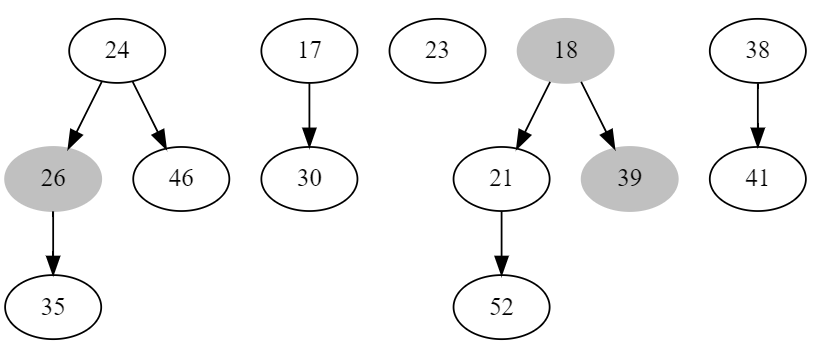
\includegraphics{C:/Users/zhuoh/Desktop/Docs/ds-18/数据结构与算法I 作业18.assets/image-20201210190459401.png}
\caption{Consolidate前}
\end{figure}

接下来,合并相同度数的节点,结果如下:

\begin{figure}
\centering
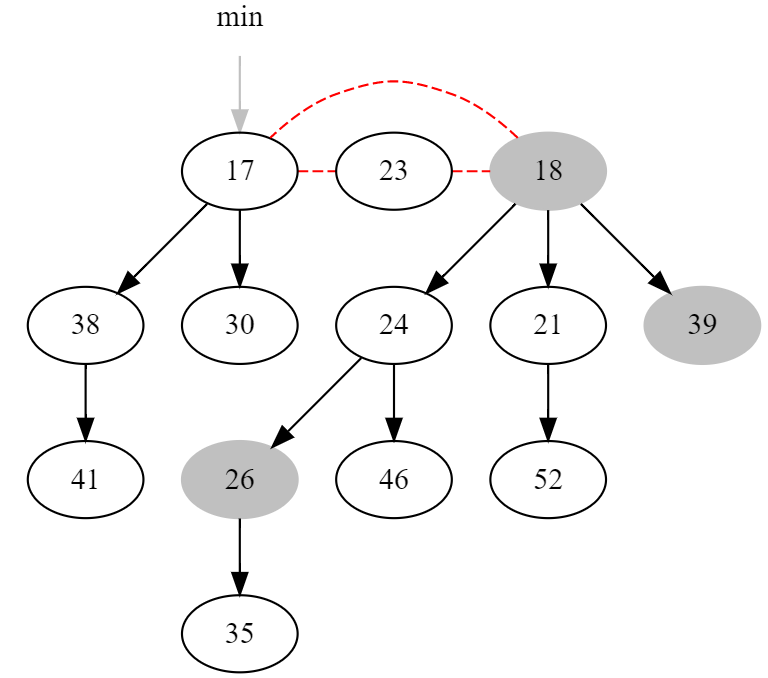
\includegraphics{C:/Users/zhuoh/Desktop/Docs/ds-18/数据结构与算法I 作业18.assets/image-20201210191315695.png}
\caption{Consolidate后}
\end{figure}

其中红色的边表示根双向链表中的连接关系,灰色节点表示被标记。

\end{document}
